
We first notice that
\begin{equation}
    \pi_1(S^n)=\pi_1(\{*\}) = \{1\}
\end{equation}
for $n\geq 2$. But clearly $S^n$ is not homotopic to the one point
space $\{*\}$, i.e. $S^n$ is not contractible! Therefore, the
fundamental homotopy group does not solve the problem of determine the
homotopy of a space. The homology groups will be an new direction to go.

The details is covered in page 173 of \cite{book}.
Sadly, even if one can computes all the homology groups (or all the
homotopy groups), one cannot determine uniquely the homotopy type of
the space in general, unless one has some additional conditions.
For example, we have the Whitehead's Theorem: Given a continuous map
from $X\to Y$, two "good" topological spaces, if $f$ induces
isomorphisms on all homotopy group $\pi_n(X)\to\pi_n(Y)$, ($n\geq 1$),
and induces bijection on $\pi_0(X)\to\pi_0(Y)$, then $f$ is a
homotopic equivalence. Is there similar good theorem for homology
groups? Perhaps there is, but it is still not good enough for we still
need to find such a $f$.

Anyway, let's proceed to the discussion of simplicial homology.
\textbf{Note}: all the following discussions are based on a given
triangulation $K$ of the space.

\subsection{Section 8.1 - Cycles and boundaries}
\label{sec:Cycles-and-boundaries}

Geometrically, the homology groups aims to encode the information
about $k$-dimensional holes in a space, as holes are important in
determining the homotopy type of a space. 

Then we notice that the boundary and bulk relation is also important.
What I mean is in the following picture. The first loop encircles
a part that does not belong to the torus, whereas the second loop
encloses a solid part in the torus. One sees that the first loop is
not nullhomotopic, i.e. it cannot be homotopic contracted to the
trivial loop. On the other hand, loop 2 can. Look more generally, if a
loop is the boundary of simple part (e.g. a simplex), then it is
homotopic to the trivial loop. In this case we physicists can regard
it as the boundary of a good bulk, g simplex. However, if a loop has
empty bulk, i.e. it encloses no simplex, it is not a boundary of
something, then it will be a nontrivial element in the fundamental
group. This is why boundaries are important in our consideration.

% todo torus-p1
\begin{figure}[H]
    \centering
    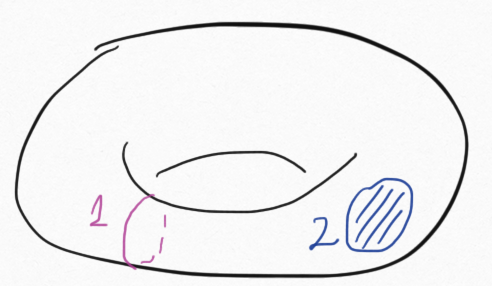
\includegraphics[width=0.6\linewidth]{pics/ch8/torus-p1.png}
\end{figure}

Before discussion, I should make clear that if we only care about
information of holes of certain dimension $q$, then we only have to care
about composition of simplexes of the same dimension $q$ that encloses
certain area (be it empty or not). For example, in fundamental groups,
we only care about holes looks like $S^1$. So in most cases we only
care about series of $1$-simplexes that is connected to form a loop,
as in the case of edge groups. We call these things that we care about
a closed $q$-cycles, to be defined precisely later.  The set of all
closed $q$-cycles are denoted $Z_q$.

Next is how to consider boundaries algebraically. For example, give a
set of vertices, how to seperate the boundary out of this? This is
especially troublesome given that we will have boundaries of different
dimensions. There are the $0$-dimension boundary of endpoints, the
$1$-dimension boundary of lines enclosing area, the $2$-dimension
boundaries called faces. 

The boundary operator $\partial$ aims to solve this problem, it gives
a systematic way to obtaining $(d-1)$-dimension boundary from a
$d$-dimension simplex. The simple examples are provided in page 174 to
175 of \cite{book}.

Lastly, as mentioned, closed $q$-cycles that is the boundary of some
solid part may become trivial, they are called $q$-boundaries. Closed
$q$-cycles that are not the boundary a solid part will be nontrivial.
Therefore, we might want to consider a quotient space:
$$ H_q = Z_q/B_q$$

I believe I have done a good job in summarizing the key point, now is
time to read the first section to get some practical ideas.

\subsection{Section 8.2 Homology groups}
\label{sec:Homology-groups}

This section formalize the intuitions from the previous section. It
defines \nomen{oriented simplex}, i.e. simplex denoted by a specific
$\{v_0,v_1,\vdots\}$ in this order. An change of order will change its
orientation. Such change of orientation is denoted by a minus sign,
and we have:
\begin{equation}
    (v_0,v_1,\cdots) = \operatorname{sign}\theta (v_{\theta(0)},
    v_{\theta(1)},\cdots)
\end{equation}
where $\theta$ is any permutation.

Then \nomen{$C_q(K)$} is the free abelian group generated by the oriented
$q$-simplexes of $K$, subject to the relations $\sigma+\tau=0$,
whenever $\sigma$ and $\tau$ are just the same simplex with opposite
orientations. An element of this group is called a \nomen{$q$-chain}.
Note that the rank of $C_q(K)$ is equal to the number of
$q$-simplexes in $K$.

The boundary homomorphism $\partial$ is defined such that
\begin{equation}
    \partial(v_0,\cdots,v_q)=\sum_{i=0}^{q}(-1)^i
    (v_{(0)},\cdots,\hat{v}_{(i)},\cdots,v_{(q)})
\end{equation}

where $(v_{(0)},\cdots,\hat{v}_{(i)},\cdots,v_{(q)})$
is shorthand for the oriented $(q-1)$-simplex obtained by deleting
the vertex $v_i$. It is easy to verify that $\partial^2=0$

In the special case when $q=0$, we define that boundary of a single
vertex is $0$ and that $C_{-1}(K)=0$.

We define the closed chains \nomen{$Z_q(K)$} as
\begin{equation}
    Z_q(K)=\Ker(\partial:C_q(K)\to C_{q-1}(K)).
\end{equation}
And the boundary \nomen{$B_q(K)$} is then
\begin{equation}
    B_q(K)=\Im(\partial:C_{q+1}(K)\to C_{q}(K)).
\end{equation}

$B_q$ will be a subgroup of $Z_q$ because $\partial^2=0$, this allows
us to define the \nomen{$q$-th homology group of $K$} as:
\begin{equation}
    H_q(K)=Z_q(K)/B_q(K)
\end{equation}

The elements of $H_q(K)$ are written $[z]$ for $z\in Z_q$, called the
\nomen{homology class} of $z$. Two $q$-cycles differ by a boundary
will have the same homology class and is called \nomen{homologous
cycles}. We note that $H_q(K)$ is by definition abelian and finitely
generated.

Of course, we need to verify various things in the above statements,
they can be found in the textbook \cite{book}.

\subsection{Section 8.3 Examples}
\label{sec:Section 8.3 Examples}

I only mention two theorems for the present:

\begin{thm}
    $H_0(K)$ is a free abelian group whose rank is the number of
    path-connected components of $|K|$ (or just components, as $|K|$
    is path-connected).
\end{thm}
\begin{proof}
    This is quite obvious.
\end{proof}

\begin{thm}
    If $|K|$ is connected, then $H_1(K)$ is isomorphic to the
    abelianization of its fundamental group $\pi_1(K)$.
\end{thm}
\begin{proof}
    Found on page 182 of \cite{book}.
\end{proof}

